% Options for packages loaded elsewhere
\PassOptionsToPackage{unicode}{hyperref}
\PassOptionsToPackage{hyphens}{url}
%
\documentclass[
]{article}
\usepackage{lmodern}
\usepackage{amssymb,amsmath}
\usepackage{ifxetex,ifluatex}
\ifnum 0\ifxetex 1\fi\ifluatex 1\fi=0 % if pdftex
  \usepackage[T1]{fontenc}
  \usepackage[utf8]{inputenc}
  \usepackage{textcomp} % provide euro and other symbols
\else % if luatex or xetex
  \usepackage{unicode-math}
  \defaultfontfeatures{Scale=MatchLowercase}
  \defaultfontfeatures[\rmfamily]{Ligatures=TeX,Scale=1}
\fi
% Use upquote if available, for straight quotes in verbatim environments
\IfFileExists{upquote.sty}{\usepackage{upquote}}{}
\IfFileExists{microtype.sty}{% use microtype if available
  \usepackage[]{microtype}
  \UseMicrotypeSet[protrusion]{basicmath} % disable protrusion for tt fonts
}{}
\makeatletter
\@ifundefined{KOMAClassName}{% if non-KOMA class
  \IfFileExists{parskip.sty}{%
    \usepackage{parskip}
  }{% else
    \setlength{\parindent}{0pt}
    \setlength{\parskip}{6pt plus 2pt minus 1pt}}
}{% if KOMA class
  \KOMAoptions{parskip=half}}
\makeatother
\usepackage{xcolor}
\IfFileExists{xurl.sty}{\usepackage{xurl}}{} % add URL line breaks if available
\IfFileExists{bookmark.sty}{\usepackage{bookmark}}{\usepackage{hyperref}}
\hypersetup{
  pdftitle={Milestone2-example},
  pdfauthor={Matthew Connell, Firas Moosvi},
  hidelinks,
  pdfcreator={LaTeX via pandoc}}
\urlstyle{same} % disable monospaced font for URLs
\usepackage[margin=1in]{geometry}
\usepackage{graphicx}
\makeatletter
\def\maxwidth{\ifdim\Gin@nat@width>\linewidth\linewidth\else\Gin@nat@width\fi}
\def\maxheight{\ifdim\Gin@nat@height>\textheight\textheight\else\Gin@nat@height\fi}
\makeatother
% Scale images if necessary, so that they will not overflow the page
% margins by default, and it is still possible to overwrite the defaults
% using explicit options in \includegraphics[width, height, ...]{}
\setkeys{Gin}{width=\maxwidth,height=\maxheight,keepaspectratio}
% Set default figure placement to htbp
\makeatletter
\def\fps@figure{htbp}
\makeatother
\setlength{\emergencystretch}{3em} % prevent overfull lines
\providecommand{\tightlist}{%
  \setlength{\itemsep}{0pt}\setlength{\parskip}{0pt}}
\setcounter{secnumdepth}{-\maxdimen} % remove section numbering
\newlength{\cslhangindent}
\setlength{\cslhangindent}{1.5em}
\newenvironment{cslreferences}%
  {\setlength{\parindent}{0pt}%
  \everypar{\setlength{\hangindent}{\cslhangindent}}\ignorespaces}%
  {\par}

\title{Milestone2-example}
\author{Matthew Connell, Firas Moosvi}
\date{05/03/2020}

\begin{document}
\maketitle

\hypertarget{autism-screening}{%
\subsection{Autism Screening}\label{autism-screening}}

\hypertarget{introduction}{%
\subsubsection{Introduction}\label{introduction}}

Autism Spectrum Disorder (ASD) is a complex neurodevelopmental condition
that impairs social interpretation/communication ability, as well as the
presence of repetitive behaviors. Current diagnostic procedures are
lengthy and inefficient (Thabtah 2019). Affecting 1.5\% of the
population, with many more cases going undetected, an easy-to-implement,
effective screening method is warranted. ASDTest, a mobile app, has been
introduced to provide an accessible screening method that tells the user
whether they should seek professional healthcare opinions, based on a 10
question survey (Allison, Auyeung, and Baron-Cohen 2012). The ability to
recognize and diagnose ASD at an early age can allow the affected to
access the healthcare resources and support they will need, in a timely
manner.

The Autism Spectrum Quotient-10
(\href{https://www.nice.org.uk/guidance/cg142/resources/autism-spectrum-quotient-aq10-test-pdf-186582493}{AQ-10})
consists of 10 questions intended to differentiate characteristics of
autism in individuals. Each question has four possible answers:
``Definitely Agree'', ``Slightly Agree,''Slightly Disagree``,
and''Definitely Disagree``. For questions 1, 5, 7, and 10, a value of 1
is assigned for either a''slightly agree" or a ``definitely agree''
response. For questions 2, 3, 4, 6, 8, and 9, a value of 1 is assigned
for either a ``slightly disagree'' or a ``definitely. disagree''
response. A cumulative score is calculated and a participant who
receives a total score of greater than 6 is recommended for a specialist
diagnostic assessment.

\hypertarget{data-description}{%
\subsubsection{Data Description}\label{data-description}}

The
\href{https://archive.ics.uci.edu/ml/datasets/Autism+Screening+Adult}{dataset}
used in this analysis was obtained from the University of California
Irvine Machine learning Repository, uploaded by Fadi Thabtah. Each row
represents an individual who participated in the survey. The survey's
results, the app's classification, and some background information about
the individual was recorded. Below is the entire variable set:

Variable

Type

Description

A1\_score

Int (0,1)

Prompt: I often notice small sounds when others do not

A2\_score

Int (0,1)

Prompt: I usually concentrate more on the whole picture, rather than the
small details

A3\_score

Int (0,1)

Prompt: I find it easy to do more than one thing at once

A4\_score

Int (0,1)

Prompt: If there is an interruption, I can switch back to what I was
doing very quickly

A5\_score

Int (0,1)

Prompt: I find it easy to `read between the lines' when someone is
talking to me

A6\_score

Int (0,1)

Prompt: I know how to tell if someone listening to me is getting bored

A7\_score

Int (0,1)

Prompt: When I'm reading a story I find it difficult to work out the
characters' intentions

A8\_score

Int (0,1)

Prompt: I like to collect information about categories of
things(e.g.~types of car, types of bird, types of train, types of plant
etc)

A9\_score

Int (0,1)

Prompt: I find it easy to work out what someone is thinking or feeling
just by looking at their face

A10\_score

Int (0,1)

Prompt: I find it difficult to work out people's intentions

Age

Int

Age of the individual

Gender

String

M (male) or F (female)

Ethnicity

String

Common Ethnicities defined for each individual

Born with Jaundice?

String (yes,no)

Was individual born with jaundice?

Country of Residence

String

Home country of individual

Used app before?

String (yes, no)

Has the user has used a screening app

Result

Int

Cumulative score of the 10 survey Q's

age\_desc

String

Age Group

relation

String

Parent, self, caregiver, medical staff, clinician ,etc.

ASD/Class

String (yes, no)

App's classification based on result

autism (Target Variable)

String (yes, no)

Does individual have an autism diagnosis?

\hypertarget{exploring-the-dataset}{%
\subsubsection{Exploring the Dataset}\label{exploring-the-dataset}}

\hypertarget{correllogram}{%
\paragraph{Correllogram}\label{correllogram}}

From the correllogram below, we can see that there's very little
correlation among any of the ten `question' variables in the dataset.
The colour scheme shows all positive correlations as blue, and all
negative correlations as red.

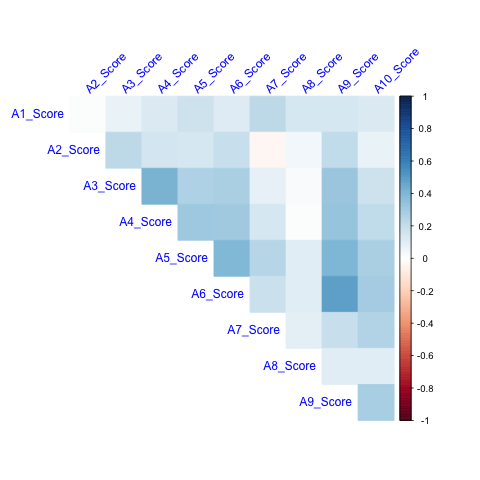
\includegraphics{../images/correlation.png}

\hypertarget{dodged-bar-chart}{%
\paragraph{Dodged Bar Chart}\label{dodged-bar-chart}}

The dodged bar chart below shows the occurences of autism in people of
different ethnicities who took the survey. This plot also illustrates an
issue with the dataset: there are two levels called `others' and one
called NA. We should definitely combine the two `others' columns and
also decide what to do about the NAs.

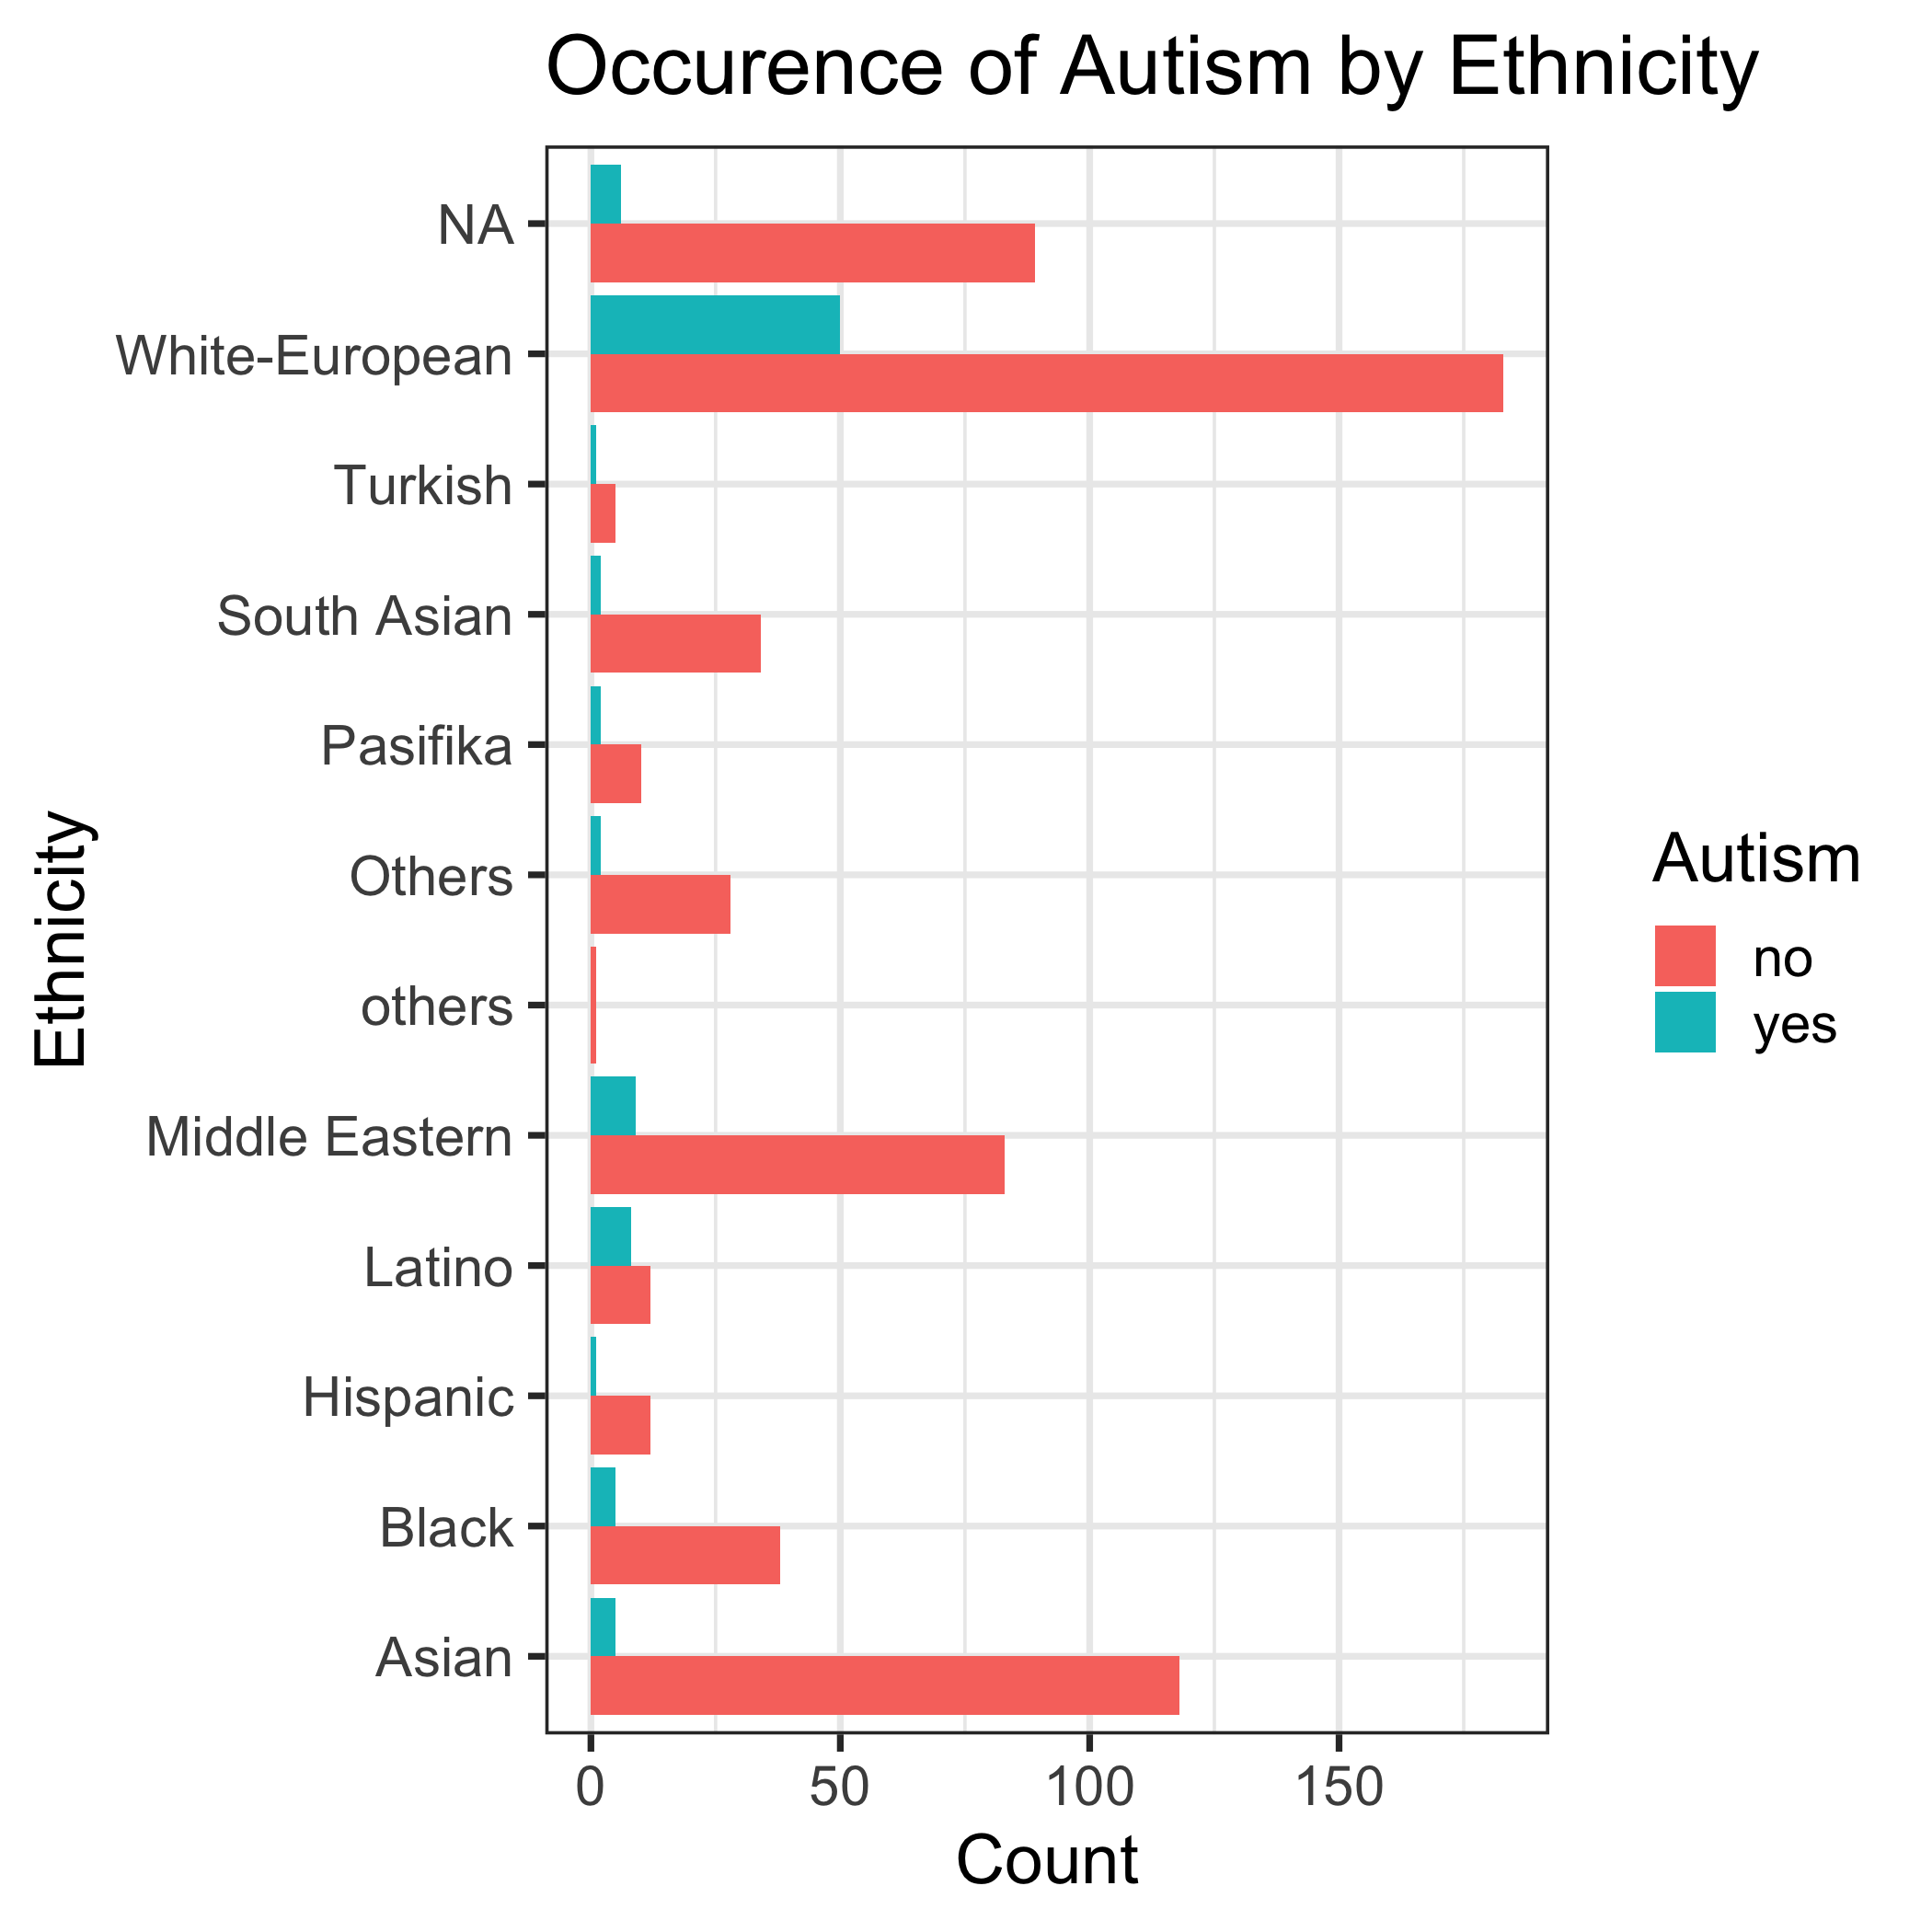
\includegraphics{../images/barplot.png}

\hypertarget{proportional-bar-chart}{%
\paragraph{Proportional Bar Chart}\label{proportional-bar-chart}}

The proportional bar chart below shows the percentage of people who were
diagnosed with autism given a particular score on the autism screening
test. A score of 0 would mean that it's incredibly unlikely the person
would be diagnosed with autism. In general, the higher the score, the
more likely it is that the person has autism.

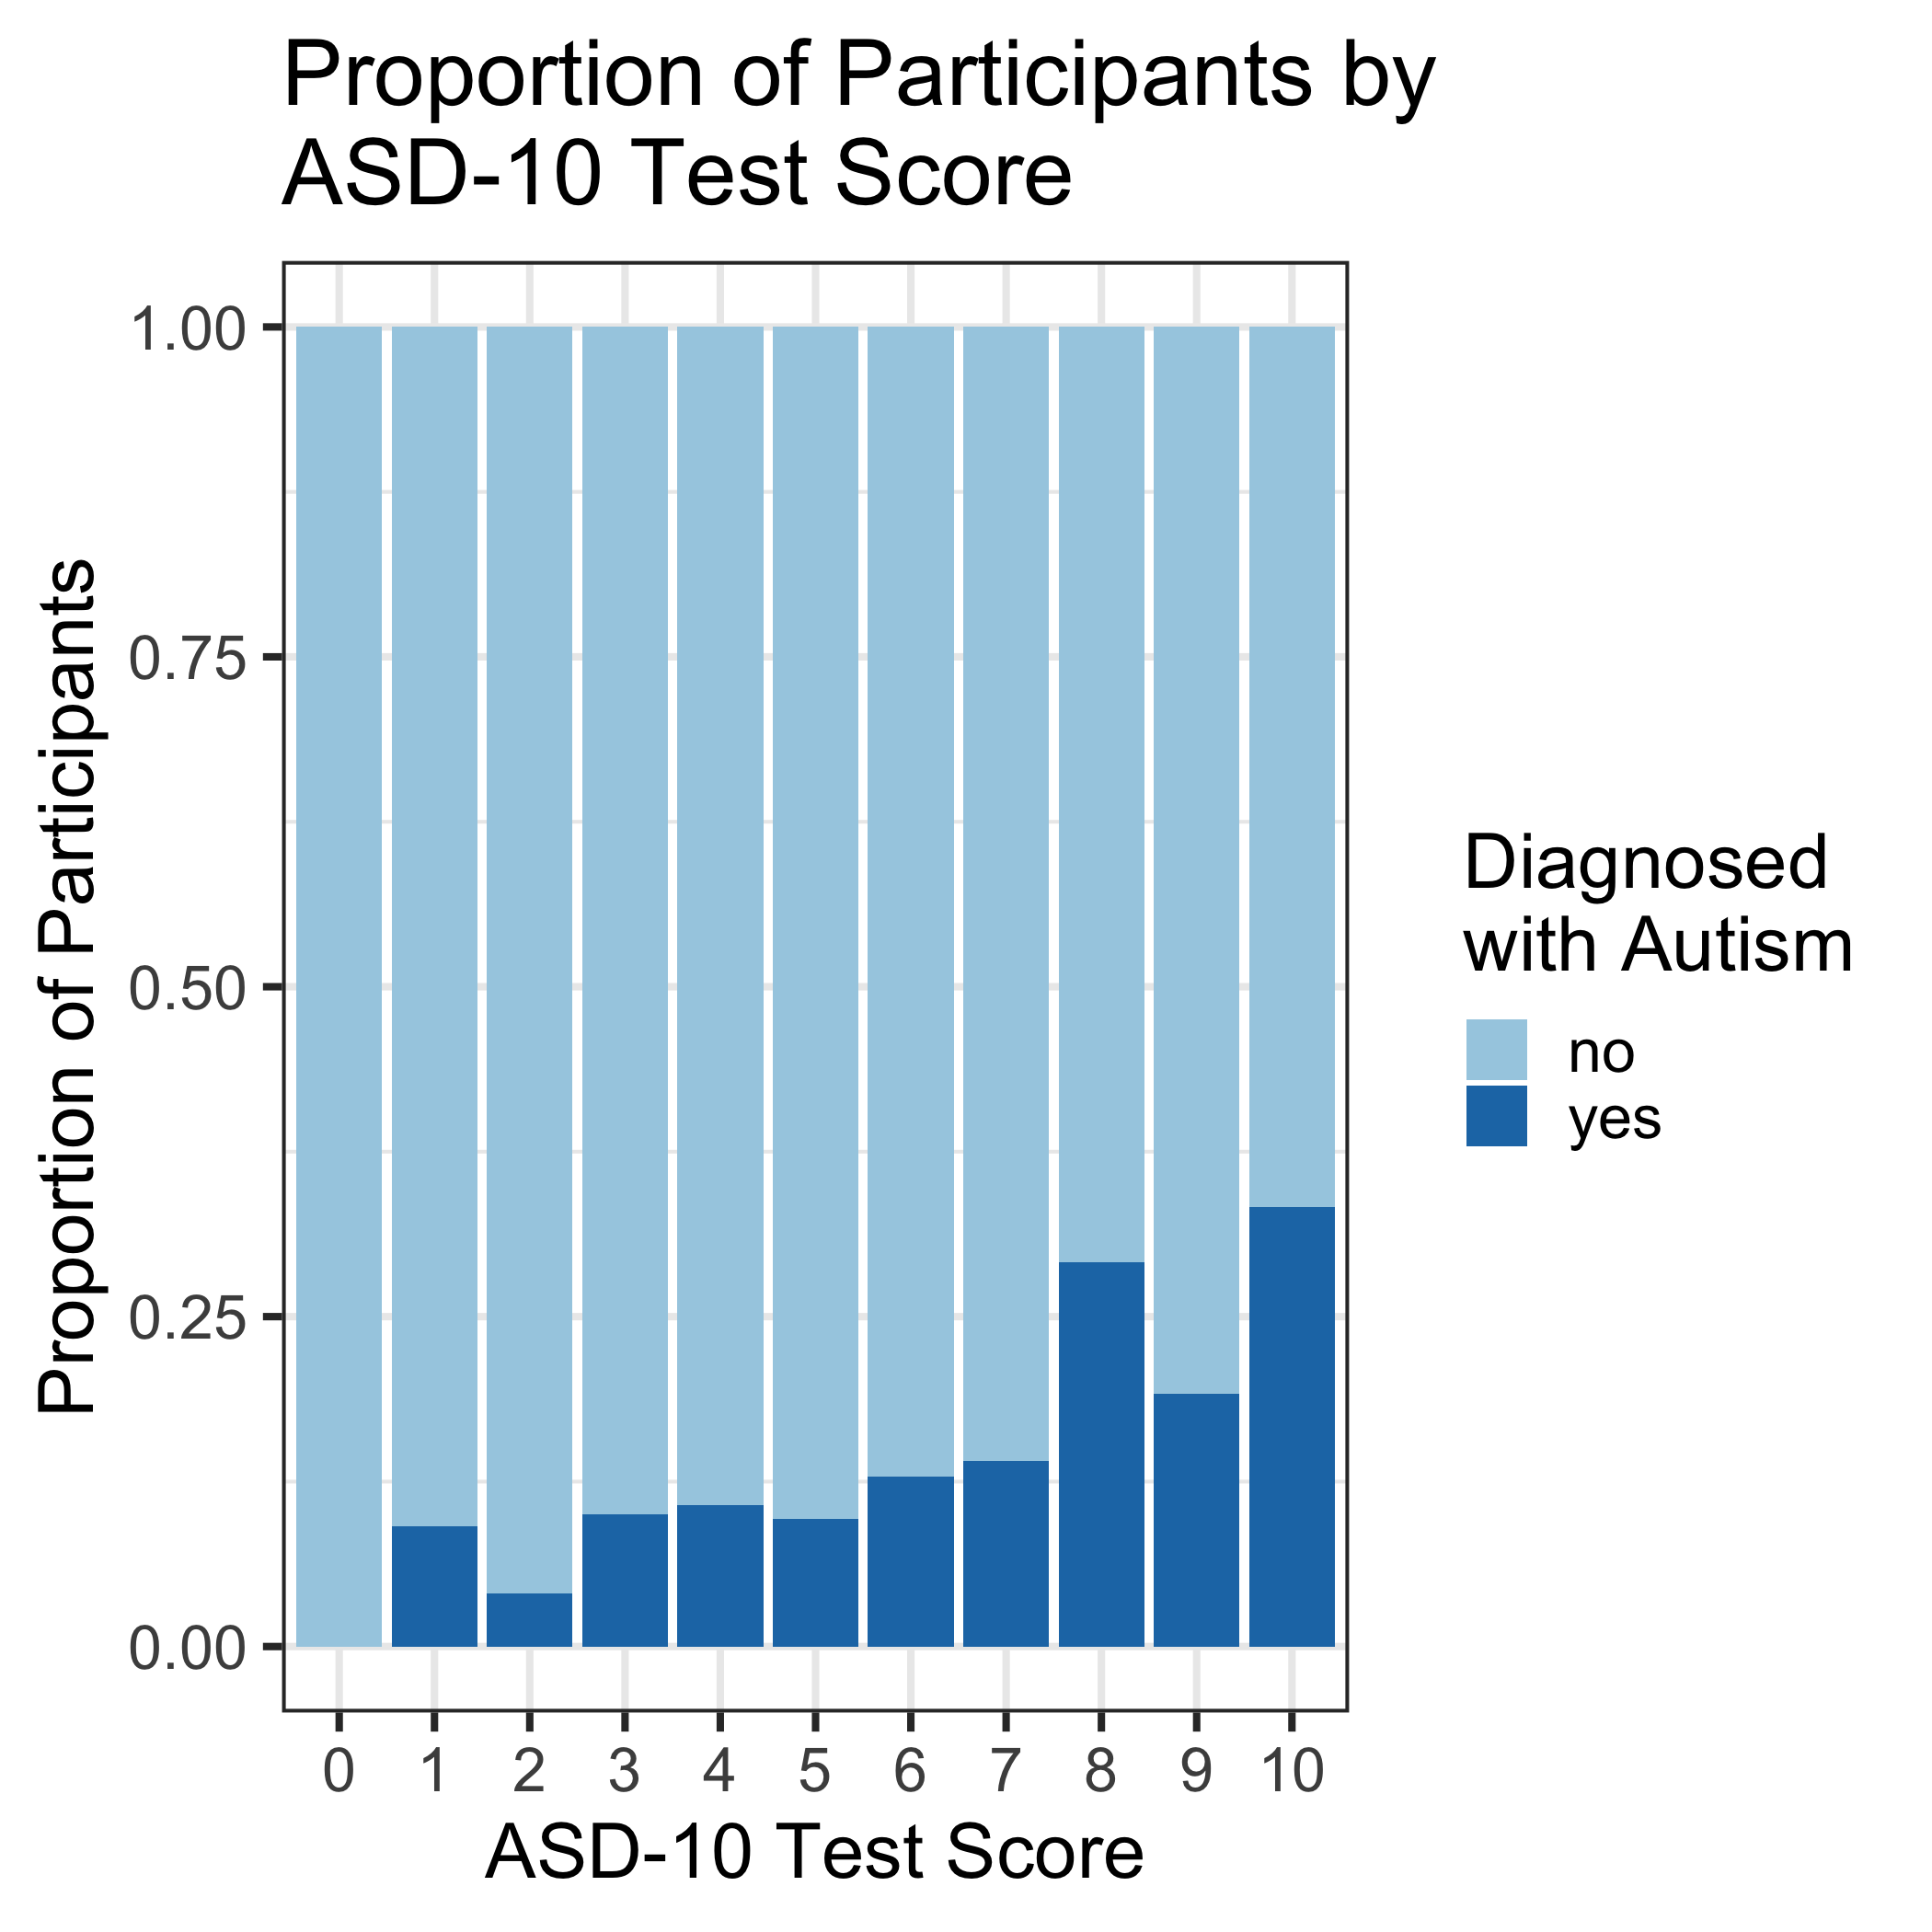
\includegraphics{../images/propbarplot.png}

\hypertarget{research-question}{%
\subsubsection{Research Question}\label{research-question}}

In this analysis, we will use logistic regression to determine the
relationship between the AQ-10 result (cumulative score) and the age of
the individual.

\hypertarget{plan-of-action}{%
\subsubsection{Plan of Action}\label{plan-of-action}}

With our research question, we are only interested in the cumulative
score and the age of the individual taking the survey. We will ignore
the other variables for the purposes of this analysis. After dealing
with the missing data, we will perform a linear regression analysis and
plot the relevant variables with a regression line.

\hypertarget{references}{%
\subsubsection{References}\label{references}}

Thomas Pin and Tejas Phaterpekar, Matthew Connell - Autism Spectrum
Disorder Screening Machine Learning Analysis -
\url{https://github.com/UBC-MDS/522-Workflows-Group-414}

\hypertarget{refs}{}
\begin{cslreferences}
\leavevmode\hypertarget{ref-allison2012toward}{}%
Allison, Carrie, Bonnie Auyeung, and Simon Baron-Cohen. 2012. ``Toward
Brief `Red Flags' for Autism Screening: The Short Autism Spectrum
Quotient and the Short Quantitative Checklist in 1,000 Cases and 3,000
Controls.'' \emph{Journal of the American Academy of Child \& Adolescent
Psychiatry} 51 (2): 202--12.

\leavevmode\hypertarget{ref-Fadi}{}%
Thabtah, Fadi. 2019. ``An Accessible and Efficient Autism Screening
Method for Behavioural Data and Predictive Analyses.'' \emph{Health
Informatics Journal} 25 (4): 1739--55.
\url{https://doi.org/10.1177/1460458218796636}.
\end{cslreferences}

\end{document}
